\documentclass{ximera, handout}  %Use handout to supress answers???
\typeout{Start loading xmPreamble.tex} %Prints message on terminal and log file. 

% Add here extra macro's that are loaded automatically by all documents of claas 'ximera' or 'xourse' in this repo 
\usepackage{tikz}
\usepackage{amsmath}
\usetikzlibrary{arrows}
\usepackage{graphicx}\usepackage{amssymb}

%\newcommand{\rulecolor}[1]{\def\CT@arc@{\color{#1}}}   %Error with Rule color when I hit serve
\definecolor{darkblue}{rgb}{0.4,0.5,0.85}
\definecolor{blue}{rgb}{0.1,0.3,.95}
%\definecolor{blue}{rgb}{0.1,0.2,0.90}
\definecolor{pink}{rgb}{0.6,0.4,0.7}
\definecolor{green}{rgb}{0.4,0.6,0.5}
\definecolor{yellow}{rgb}{0.1,0.6,0.8}
\definecolor{red}{rgb}{0.8,0.1,0.5}
\definecolor{glaucous}{rgb}{0.38,0.51,0.71}

\usepackage{pgfplots}
\pgfplotsset{compat=1.16}
\usetikzlibrary{calc,angles,positioning,intersections,quotes,decorations.markings}
\pgfplotsset{soldot/.style={only marks,mark=*, line width=0.2pt, mark size=1.5pt}}
\pgfplotsset{holdot/.style={fill=white,only marks,mark=*, line width=1.0pt, mark size=1.5pt}}


\usepackage[utf8]{inputenc}  %needed to define \begin{axis} in tikz pic

%%
%%  Example:
%%
% \newcommand{\R}{\mathbb{R}


\title{Collection of Activities}
\author{Kelly Stady}

\begin{document}
\begin{abstract}
    Practice Problems
\end{abstract}
\maketitle


\begin{exercise}
    \[ 2+10=\answer{12} \]
\end{exercise}


\begin{exercise}
Find the limit if $f(x) = x.$ 

\[ \lim\limits_{x \to 2} f(x) = \answer{2} \]

%\[
%\lim\limits_{x \to 2} f(x)
%\]
\end{exercise}

\begin{question}
    The circle below has been divided into 10 equal parts.  What fraction of the circle is shaded? \\ \\


   \begin{center}  %Makes circle huge!!  scale=0.1 does not help
   \hspace{0.8in} 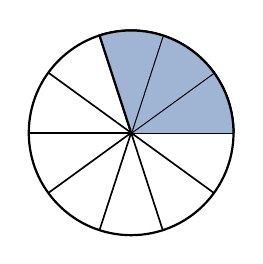
\begin{tikzpicture}
   \draw[thick] (0,0) circle [radius=1.3cm];
   \foreach \i in {36,72,...,360}
    \draw[semithick] (0,0)--(\i:1.3cm);    %The colon signifies that polar coordinates are being used. (60:.75cm) means the point that is at an angle of 60° and a distance of 0.75cm from the origin. Length of radial lines - should match radius above.
    \draw[thick, fill=glaucous!60] (0,0) --  (36:1.3) arc(36:0:1.3); %To Draw Arc: \draw (x,y) arc (start:stop:radius);
    \draw[thick, fill=glaucous!60] (0,0) --  (72:1.3) arc(72:36:1.3); %Colon indicates polar coordintes (angle:length)
    \draw[thick, fill=glaucous!60] (0,0) --  (108:1.3) arc(108:72:1.3);
    %\draw[fill=glaucous] (0,0) -- (360:1.5) arc(360:324:1.5);
     \end{tikzpicture}
     \end{center}

    \begin{multipleChoice}
   \choice[correct]{$\displaystyle \frac{3}{10}$}
   \choice{$\displaystyle \frac{1}{10}$}
   \choice{$\displaystyle \frac{7}{10}$}
   \end{multipleChoice}  
   \end{question}  



%\begin{center} %% Image is found in xmPictures
%
\includegraphics{missionPatch.jpg}
%\end{center}




%%%%%%%%%%%%%%%%%%%%%%%%%%%%%%%%%%%%%%%%%%%%%%%%%%%%%%%%%%%%%%%
\begin{itemize}
    \item Calculus was discovered in the seventeenth century by
    Leibniz and Newton, independently.  The development of calculus was
    motivated in large part by two geometric problems: 
    
    \begin{enumerate}
    \item Finding areas of plane regions.
    
    \item Finding tangent lines to curves.
    \end{enumerate}
    
    
    \vspace{0.1in}
    \item \textbf{The Tangent Line Problem}
    
    In algebra you learned how to find the slope of a line, which
    measures the change in $y$ for a given change in $x.$ For example,
    a slope of $m=-\frac{32}{1}$ indicates that when $x$ increases by
    1, the value of $y$ decreases by 32. The slope of a line is also a
    measure of the steepness of the line and is constant. Intuitively,
    we know that the steepness of a curve is \emph{not} constant.  So
    how do we measure the steepness or slope of a curve at a
    particular point? \\ \\ 
    
    \vspace{0.1in} We draw a line that touches the curve at the point.
    This line is called a \textbf{tangent line}. The tangent line and
    curve have this point in common, so we define the slope of the
    curve at this point to be the slope of the tangent line. \\ \\
    
    \vspace{0.2in} 
    \item[]\textbf{The slope of a curve at  a point is equal to the slope of the tangent line at that point}. \\  \\
    

    \vspace{0.2in}
    \item[] Below is the graph of $y=e^x$ along
    with its tangent line at $x=1.2.$  To find the slope of the tangent line, we need to
    know two points that lie on the line, but we only know one $(1.2,
    e^{1.2}).$ In the next chapter, we will see how to find the slope
    of the tangent line without finding a second point on the line.
    This process involves finding a limit, which is the focus of this
    section.
    
    %with(Student[Calculus1])
    %z:= plots[pointplot]([1.2, exp(1.2)], symbol = solidcircle, color = black, symbolsize = 23)
    %z2:= plot([exp(x), Tangent(exp(x), x = 1.2, showpoint = true)], x = -4 .. 4, -5 .. 10, color = [black, black], linestyle = [1, 3], thickness = 3, labelfont = [COURIER, 1], axesfont = ["HELVETICA", "COMPUTER MODERN", 17])
    %display({z, z2})
    
    %Old
    %with(Student[Calculus1][Tangent])
    %plot([exp(x), Tangent(exp(x), x = 1.2, output = line)], x = -4 .. 4, -5 .. 10, color = [black, black], linestyle = [1, 3], thickness = 2)
    
    
    \vspace{0.1in}
    
    \hspace{0.4in}
    %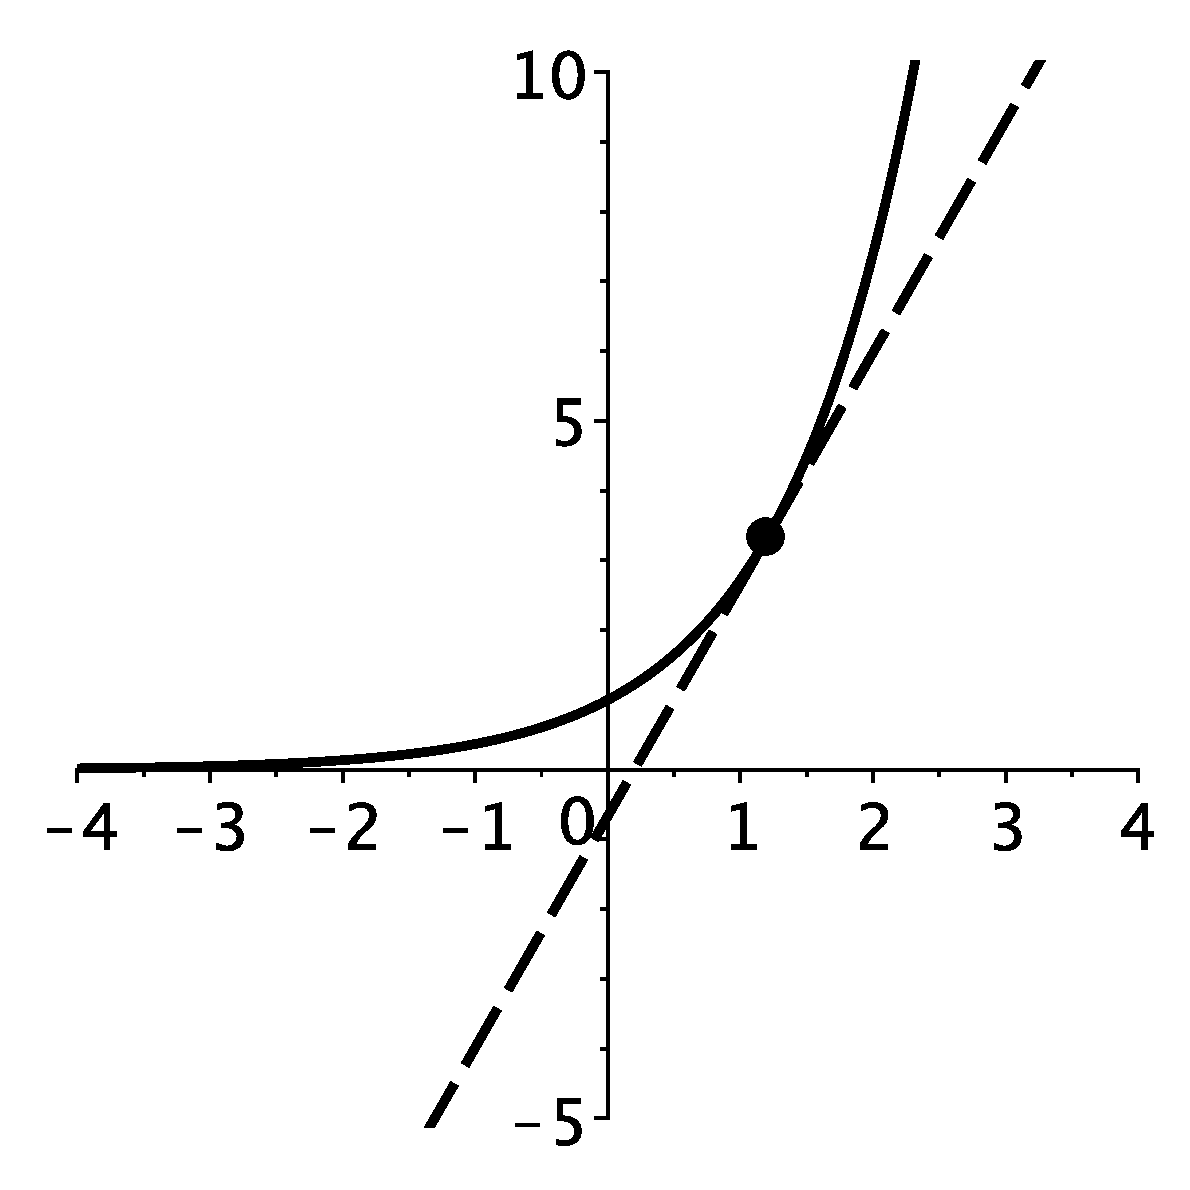
\includegraphics[height=2in, width=2in]{plot1s22.eps}
    
    
    \vspace{0.2in}
    \item The most basic use of \textbf{limits} is to
    describe how a function $y=f(x)$ behaves as $x$ approaches a
    particular value.
    
    
    
    \newpage
    \fbox{\parbox{6.2in}{\textbf{\fbox{\parbox{6.1in}{\textbf{Limit Notation}}}}
    
    \vspace{0.1in}
    The \textbf{limit of a function} $y=f(x)$ is the value that $f(x)$
    approaches as $x$ approaches a fixed value $c.$  The value of
    the limit is commonly denoted by $L$.  The mathematical notation
    for limits is given below.
    \[ \lim_{x \rightarrow c} f(x) = L \hspace{0.5in} \small{\textrm{Read as:} \ ``\textrm{\textbf{The limit of} $f(x)$ \textrm{\textbf{as}} $x$
    \textrm{\textbf{approaches}} $c$ is $L$."}} \] }}
    
    \textbf{Remark:} This notation allows us to mathematically describe the behavior of a function around a point at
    which it is undefined or discontinuous.  It also allows us to describe the end behavior of the function, that is how does
    the function behave as $x \rightarrow \pm \infty$.
    
    
    \vspace{0.2in} \item[$\bigstar$] \textbf{Problem I:} \ Use a limit
    to describe the behavior of the function $f(x)=\ln x$ as $x$
    approaches $1.$




    \begin{definition}\index{limits}
    The \textbf{limit of a function} $f(x)$ is the value that $f(x)$
    approaches as $x$ approaches a fixed value $c.$  The value of
    the limit is commonly denoted by $L$.  The mathematical notation
    for limits is given below.
    \[ \lim_{x \rightarrow c} f(x) = L  \] 
      \end{definition}

\end{itemize}

\end{document}
